% =================================================================
%  ALIGN paper — Figure sketches
%  Compile with:  pdflatex figure_sketches.tex
%  Author: ALIGN team, 2026-07-30
%
%  This file contains two standalone figures for the ALIGN paper:
%    - fig:venn     (Section 1) — Venn diagram of three lineages
%    - fig:treemap  (Section 2) — Tree map of related work
%
%  Both figures share a common color scheme (Okabe-Ito) and are
%  self-contained — no external files required.
% =================================================================
\documentclass[11pt]{article}

\usepackage[a4paper, margin=1in]{geometry}
\usepackage{microtype}
\usepackage{xcolor}
\usepackage{tikz}
\usepackage{forest}
\usepackage{amsmath}
\usepackage{booktabs}
\usepackage{hyperref}

% --- Okabe-Ito colorblind-safe palette ---
\definecolor{okblue}{HTML}{0072B2}
\definecolor{okorange}{HTML}{E69F00}
\definecolor{okgreen}{HTML}{009E73}
\definecolor{okred}{HTML}{D55E00}
\definecolor{okpurple}{HTML}{CC79A7}
\definecolor{okcyan}{HTML}{56B4E9}
\definecolor{okyellow}{HTML}{F0E442}
\definecolor{okgray}{HTML}{999999}

\usetikzlibrary{arrows.meta, positioning, shapes.geometric, calc, fit, backgrounds, shadows}

\title{ALIGN paper — Figure Sketches\\
  \large Venn diagram + Tree map for Related Work}
\author{ALIGN team}
\date{July 30, 2026}

\begin{document}
\maketitle

% =================================================================
\section*{Figure 1: Venn diagram of three lineages}
% =================================================================

\noindent\textbf{Purpose:} To communicate at a glance that ALIGN is the
first architecture occupying the 3-way intersection of autonomous
manipulation, shared autonomy, and task-semantic extraction.

\begin{figure}[h]
\centering
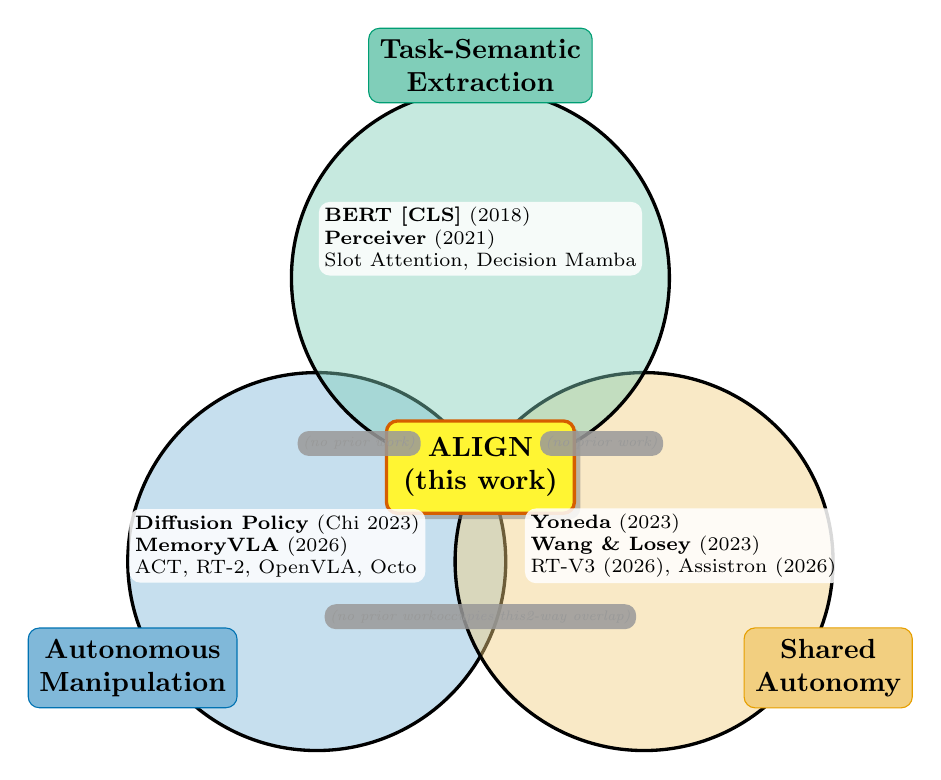
\begin{tikzpicture}[
    every node/.style={font=\small},
    circ/.style={draw, very thick, fill opacity=0.45, text opacity=1,
                 line width=1.2pt},
    circA/.style={circ, fill=okblue!50},
    circB/.style={circ, fill=okorange!50},
    circC/.style={circ, fill=okgreen!50},
    align centered/.style={align=center},
]
% --- Three circles (equilateral layout) ---
% Place circle centers at 120-degree angles around the figure center.
\def\R{2.4}                              % circle radius
\def\RC{2.4}                             % distance from figure center to circle center

% Compute centers using polar coords (top-left, top-right, bottom)
\coordinate (figC)   at (0, 0);          % figure center
\coordinate (cA)     at (210:\RC);       % Autonomous Manipulation (bottom-left)
\coordinate (cB)     at (330:\RC);       % Shared Autonomy (bottom-right)
\coordinate (cC)     at (90:\RC);        % Task-semantic Extraction (top)

\draw[circA] (cA) circle (\R);
\draw[circB] (cB) circle (\R);
\draw[circC] (cC) circle (\R);

% --- Circle labels (placed outside) ---
\node[font=\bfseries, fill=okblue!50, draw=okblue, rounded corners,
      inner sep=4pt, align=center]
    at ($(cA)+(210:2.7)$) {Autonomous\\Manipulation};

\node[font=\bfseries, fill=okorange!50, draw=okorange, rounded corners,
      inner sep=4pt, align=center]
    at ($(cB)+(330:2.7)$) {Shared\\Autonomy};

\node[font=\bfseries, fill=okgreen!50, draw=okgreen, rounded corners,
      inner sep=4pt, align=center]
    at ($(cC)+(90:2.7)$) {Task-Semantic\\Extraction};

% --- ALIGN: at the 3-way overlap (figure center) ---
\node[draw=okred, very thick, fill=yellow!80, rounded corners,
      inner sep=6pt, align=center, font=\bfseries, drop shadow]
    at (figC) {ALIGN\\(this work)};

% --- Prior works listed inside each lineage's exclusive region ---
\node[align=left, font=\scriptsize, fill=white, fill opacity=0.85, text opacity=1,
      inner sep=2pt, rounded corners]
    at ($(cA)+(-0.5, 0.2)$)
    {\textbf{Diffusion Policy} (Chi 2023)\\
     \textbf{MemoryVLA} (2026)\\
     ACT, RT-2, OpenVLA, Octo};

\node[align=left, font=\scriptsize, fill=white, fill opacity=0.85, text opacity=1,
      inner sep=2pt, rounded corners]
    at ($(cB)+(0.5, 0.2)$)
    {\textbf{Yoneda} (2023)\\
     \textbf{Wang \& Losey} (2023)\\
     RT-V3 (2026), Assistron (2026)};

\node[align=left, font=\scriptsize, fill=white, fill opacity=0.85, text opacity=1,
      inner sep=2pt, rounded corners]
    at ($(cC)+(0, 0.5)$)
    {\textbf{BERT [CLS]} (2018)\\
     \textbf{Perceiver} (2021)\\
     Slot Attention, Decision Mamba};

% --- Pairwise intersections: claim "no prior work" ---
\node[font=\tiny\itshape, fill=white, fill opacity=0.85, text opacity=1,
      inner sep=2pt, rounded corners, color=okgray]
    at ($(cA)!0.5!(cB)+(0,-0.7)$)
    {(no prior work\\occupies this\\2-way overlap)};

\node[font=\tiny\itshape, fill=white, fill opacity=0.85, text opacity=1,
      inner sep=2pt, rounded corners, color=okgray]
    at ($(cA)!0.5!(cC)+(-0.5,-0.3)$)
    {(no prior work)};

\node[font=\tiny\itshape, fill=white, fill opacity=0.85, text opacity=1,
      inner sep=2pt, rounded corners, color=okgray]
    at ($(cB)!0.5!(cC)+(0.5,-0.3)$)
    {(no prior work)};
\end{tikzpicture}
\caption{ALIGN is the first architecture that simultaneously occupies
three lineages: autonomous manipulation (Chi 2023, MemoryVLA 2026),
shared autonomy (Yoneda 2023, Wang \& Losey 2023, RT-V3 2026,
Assistron 2026), and task-semantic extraction (BERT 2018, Perceiver
2021, Slot Attention, Decision Mamba 2024). No prior work occupies
even any of the 2-way overlaps.}
\label{fig:venn}
\end{figure}

% =================================================================
\section*{Figure 2: Tree map of related work}
% =================================================================

\noindent\textbf{Purpose:} To enumerate the related-work landscape
organized by lineage, with ALIGN highlighted at the unique 3-way overlap.

\begin{figure}[h]
\centering
\begin{forest}
for tree={
    grow'=east,                     % branches grow rightward
    parent anchor=east,
    child anchor=west,
    edge path={
        \noexpand\path [draw, \forestoption{edge}]
        (!u.parent anchor) -| +(8pt,0) |- (.child anchor)\forestoption{edge label};
    },
    anchor=west,
    align=left,
    l sep=8pt,
    s sep=4pt,
    inner xsep=2pt,
    inner ysep=2pt,
    font=\small,
    where level=0{
        font=\bfseries\large,
        fill=okgray!30,
        draw=okgray,
        rounded corners=2pt,
        inner xsep=6pt,
    }{},
    where level=1{
        font=\bfseries,
        rounded corners=2pt,
    }{},
    where level=2{
        font=\itshape\small,
    }{},
    where level=3{
        font=\scriptsize,
        fill=white,
    }{},
    % Color the three top-level lineages
    delay={
        tempcounta'=0,
        for tree={
            if level=1{
                if={\strcmp{\forestoption{content}}{Autonomous Manipulation}}{content={Autonomous\\Manipulation}}{},
                if={\strcmp{\forestoption{content}}{Shared Autonomy}}{content={Shared\\Autonomy}}{},
                if={\strcmp{\forestoption{content}}{Task-Semantic Extraction}}{content={Task-Semantic\\Extraction\\(from RNN/SSM)}}{},
            }{},
        },
    },
    % Highlight ALIGN
    highlight/.style={
        fill=yellow!80,
        draw=okred,
        very thick,
        edge={okred, very thick, dashed},
        edge label={node[midway, font=\tiny\bfseries, fill=white,
                            inner sep=1pt, rounded corners]{3-way\\overlap}},
    },
}
[Robotics, tikz={\node[draw=none, fill=none] at () {Robotics};}
  [{Autonomous\\Manipulation}, fill=okblue!25, draw=okblue, thick,
    [{Imitation\\learning}, fill=okblue!15,
      [{BC, ACT\\Diffusion Policy\\(Chi 2023)\\RT-2, RT-X}]
    ]
    [{Foundation\\VLAs}, fill=okblue!15,
      [{OpenVLA, Octo\\π$_0$, GR-1}]
    ]
    [{Memory-\\augmented}, fill=okblue!15,
      [{MemoryVLA (2026)\\RAG-policy}]
    ]
  ]
  [{Shared\\Autonomy}, fill=okorange!25, draw=okorange, thick,
    [{Goal\\inference}, fill=okorange!15,
      [{POMDP (Javdani)\\Visual goal\\quad (Jonnavittula)\\VLM-mediated\\quad (Casper, SAFe-Copilot)}]
    ]
    [{Arbitration}, fill=okorange!15,
      [{$α$-blending\\quad (Wang \& Losey)\\Forward-reverse\\quad (Yoneda)\\Bayesian posterior\\quad (RT-V3)\\Flow-match guidance\\quad (Assistron)}]
    ]
    [{Adaptive $α$}, fill=okorange!15,
      [{SA-DRL (Reddy)\\Atan (2024)\\Lima MPC (2024)}]
    ]
  ]
  [{Task-Semantic\\Extraction}, fill=okgreen!25, draw=okgreen, thick,
    [{Fixed query\\+ attention}, fill=okgreen!15,
      [{BERT [CLS] (2018)\\Perceiver IO (2021)\\Slot Attention (2020)\\Set Transformer (2019)}]
    ]
    [{Fixed query\\+ RNN/SSM}, fill=okgreen!15,
      [{Decision Mamba (2024)\\Prompt-DT (Xu 2022)\\LPDT (Yang \& Xu)}]
    ]
    [{Multimodal\\grounding}, fill=okgreen!15,
      [{CLIP (Radford 2021)\\ALIGN (Caron 2021)\\Language-as-supervision}]
    ]
  ]
  [{\bfseries ALIGN\\(this work)}, highlight,
  ]
]
\end{forest}
\caption{Related work organized into three lineages.
\textbf{Autonomous manipulation} (blue) — diffusion policy, VLA, memory-augmented.
\textbf{Shared autonomy} (orange) — goal inference, arbitration, adaptive $α$.
\textbf{Task-semantic extraction} (green) — fixed learnable queries over
attention or recurrent state, with multimodal grounding.
ALIGN is the only work spanning all three; it is highlighted at the
3-way overlap.}
\label{fig:treemap}
\end{figure}

\newpage
% =================================================================
\section*{Figure 1 (variant): Linear taxonomy + ALIGN cross-references}
% =================================================================

\noindent\textbf{Purpose:} A simpler alternative to the Venn diagram
for slides or talks. Each lineage is a row; ALIGN appears as a vertical
band that crosses all three.

\begin{figure}[h]
\centering
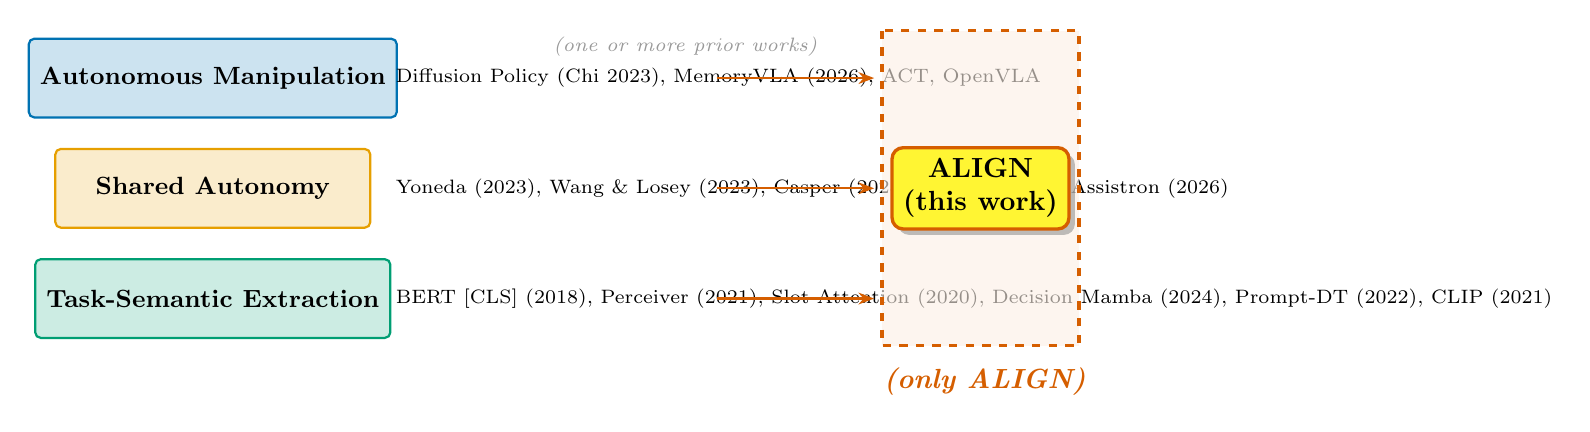
\begin{tikzpicture}[
    every node/.style={font=\small},
    row/.style={rectangle, rounded corners=2pt, draw, thick,
                minimum height=1.0cm, inner sep=4pt},
    align centered/.style={align=center},
]
% Three rows for the three lineages
\node[row, fill=okblue!20, draw=okblue, minimum width=4cm]
    at (0, 0) {\bfseries Autonomous Manipulation};
\node[row, fill=okorange!20, draw=okorange, minimum width=4cm]
    at (0, -1.4) {\bfseries Shared Autonomy};
\node[row, fill=okgreen!20, draw=okgreen, minimum width=4cm]
    at (0, -2.8) {\bfseries Task-Semantic Extraction};

% Prior works listed inside each row
\node[align=left, font=\scriptsize, anchor=west] at (2.2, 0)
    {Diffusion Policy (Chi 2023), MemoryVLA (2026), ACT, OpenVLA};
\node[align=left, font=\scriptsize, anchor=west] at (2.2, -1.4)
    {Yoneda (2023), Wang \& Losey (2023), Casper (2025), RT-V3 (2026),
     Assistron (2026)};
\node[align=left, font=\scriptsize, anchor=west] at (2.2, -2.8)
    {BERT [CLS] (2018), Perceiver (2021), Slot Attention (2020),
     Decision Mamba (2024), Prompt-DT (2022), CLIP (2021)};

% ALIGN: vertical band crossing all three rows
\draw[okred, very thick, dashed, fill=okred!10, fill opacity=0.6]
    (8.5, 0.6) rectangle (11, -3.4);
\node[draw=okred, very thick, fill=yellow!80, rounded corners,
      align=center, font=\bfseries, drop shadow, inner sep=4pt]
    at (9.75, -1.4) {ALIGN\\(this work)};

% Arrows from each lineage into ALIGN band
\foreach \y in {0, -1.4, -2.8} {
    \draw[-{Stealth[length=2mm]}, okred, thick]
        (6.4, \y) -- (8.4, \y);
}

% Caption labels
\node[font=\scriptsize\itshape, color=okgray, anchor=west]
    at (4.2, 0.4) {(one or more prior works)};
\node[font=\bfseries\itshape, color=okred, anchor=west]
    at (8.4, -3.85) {(only ALIGN)};

\end{tikzpicture}
\caption{Linear taxonomy of related work. ALIGN (right band) is the
only architecture that crosses all three lineages. Each prior work
sits in one (or sometimes two) lineages but never all three.}
\label{fig:linear}
\end{figure}

\end{document}
